% To do:
% Perplexity details, Word Error Rate for training (method section).
% The norm of different layers after training and before training
% Our framework is flexible. (abstract?)
% Do we need to say more about the R@5, R@10 for flickr-30K? (experiment)
% Details of the training: (model description? exp? prefer experiments)
%  1. Number of words in the dictionary
%  2. Word error rate
%  3. Training time
% Finetuning the networks? (future works)

\section{Experiments}

\subsection{Datasets}
We test our method on three benchmark datasets with sentence level annotations: IAPR TC-12 \cite{grubinger2006iapr}, Flickr 8K \cite{rashtchian2010collecting}, and Flickr 30K \cite{hodoshimage}.

% Here are some statistics and our experimental settings for the three datasets:

\textbf{IAPR TC-12 Benchmark}.
This dataset consists of around 20,000 images taken from locations around the world.
This includes images of different sports and actions, people, animals, cities, landscapes, and so on.
For each image, they provide at least one sentence annotation.
On average, there are about 1.7 sentences annotations for one image.
We adopt the publicly available separation of training and testing set as previous works \cite{GVS10a,kiros2013multimodal}.
There are 17,665 images for training and 1962 images for testing.

\textbf{Flickr8K Benchmark}.
This dataset consists of 8,000 images extracted from Flickr.
For each image, it provides five sentences annotations.
The grammar of the annotations for this dataset is simpler than that for the IAPR TC-12 dataset.
We adopt the standard separation of training, validation and testing set which is provided by the dataset.
There are 6,000 images for training, 1,000 images for validation and 1,000 images for testing.

\textbf{Flickr30K Benchmark}.
This dataset is a recent extension of Flickr8K.
For each image, it also provides five sentences annotations.
It consists of 158,915 crowd-sourced captions describing 31,783 images.
The grammar and style for the annotations of this dataset is similar to Flickr8K.
We follow the previous work \cite{karpathy2014fragment} which used 1,000 images for testing.
This dataset, as well as the Flick8K dataset, are commonly used for the image-sentence retrieval tasks.
%and there is not public available results of methods for generating novel sentence descriptions.

\subsection{Evaluation metrics}
\label{sec:EvaRet}

\textbf{Sentence Generation}.
Following previous works, we adopt sentence perplexity and BLEU scores (i.e. B-1, B-2, and B-3) \cite{papineni2002bleu,lin2004automatic} as the evaluation metrics.
BLEU scores were originally designed for automatic machine translation where they rate the quality of a translated sentences given several references sentences.
We can treat the sentence generation task as the ``translation'' of the content of images to sentences.
BLEU remains the standard evaluation metric for sentence generation methods for images, though it has drawbacks.
For some images, the reference sentences might not contains all the possible descriptions in the image and BLEU might penalize some correctly generated sentences. 
To conduct a fair comparison, we adopt the same sentence generation steps and experiment settings as \cite{kiros2013multimodal}, and generate as many words as there are in the reference sentences to calculate BLEU.
Note that our model does not need to know the length of the reference sentence because we add a end sign "\#\#END\#\#" at the end of every training sentences and we can stop the generation process when our model outputs the end sign.

\textbf{Sentence Retrieval and Image Retrieval}
For Flickr8K and Flickr30K datasets, we adopted the same evaluation metrics as previous works \cite{socher2014grounded,frome2013devise,karpathy2014fragment} for both the tasks of sentences retrieval and image retrieval.
They used R@K (K = 1, 5, 10) as the measurements, which are the recall rates of the first retrieved groundtruth sentences (sentence retrieval task) or images (image retrieval task).
Higher R@K usually mean better retrieval performance.
Since we care most about the top-ranked retrieved results, the R@K with small K are more important.
The Med r is another score we used, which is the median rank of the first retrieved groundtruth sentences or images.
Lower Med r usually means better performance.

For IAPR TC-12 datasets, we adopt exactly the same evaluation metrics as \cite{kiros2013multimodal} and plot the mean number of matches of the retrieved groundtruth sentences or images with respect to the percentage of the retrieved sentences or images for the testing set.
For sentences retrieval task, \cite{kiros2013multimodal} used a shortlist of 100 images which are the nearest neighbors of the query image in the feature space.
This shortlist strategy makes the task harder because similar images might have similar descriptions and it is often harder to find  subtle differences among the sentences and pick the most suitable one.
Although there are no published R@K scores and Med r score for this dataset available for the best of our knowledge, we also report these scores of our method for future comparison.

\subsection{Results on IAPR TC-12}

\begin{table}[htb]
	\centering
\begin{tabular}{l|cccc}
\hline
      & $\mathcal{PPL}$  & B-1   & B-2   & B-3 \\
\hline
BACK-OFF GT2 & 54.5  & 0.323 & 0.145 & 0.059 \\
BACK-OFF GT3 & 55.6  & 0.312 & 0.131 & 0.059 \\
LBL \cite{mnih2007three}  & 20.1  & 0.327 & 0.144 & 0.068 \\
MLBL-B-DeCAF \cite{kiros2013multimodal} & 24.7  & 0.373 & \textbf{0.187} & 0.098 \\
MLBL-F-DeCAF \cite{kiros2013multimodal} & 21.8  & 0.361 & 0.176 & 0.092 \\
Gupta et al. \cite{gupta2012choosing} & /     & 0.15  & 0.06  & 0.01 \\
Gupta \& Mannem \cite{gupta2012image} & /     & 0.33  & 0.18  & 0.07 \\
\hdashline
Ours-RNN-Base & 7.77  & 0.3134 & 0.1168 & 0.0803 \\
Ours-m-RNN & \textbf{6.92} & \textbf{0.3951} & 0.1828 & \textbf{0.1311} \\
\hline
\end{tabular}%
	\caption{Results of the sentence generation task on the IAPR TC-12 dataset. ``B'' is short for BLUE}
	\label{tab:iaprtc_gen}
\end{table}

The results of the sentence generation task are shown in Table \ref{tab:iaprtc_gen}.
BACK-OFF GT2 and GT3 are n-grams methods with Katz backoff and Good-Turing discounting \cite{chen2000survey,kiros2013multimodal}.
Ours-RNN-Base serves as a baseline method for our m-RNN model.
It has the same architecture with m-RNN except that we will not input the image features to the network.

To conduct a fair comparison, we followed the same experimental settings of \cite{kiros2013multimodal}, include the context length to calculate the BLEU scores and perplexity.
These two evaluation metrics are not necessarily correlated to each other for the following reasons.
As mentioned in Section \ref{sec:trainCost}, perplexity is calculated according to the conditional probability of the word in a sentence given all of its previous reference words.
Therefore, a strong language model that successfully captures the distributions of words in sentences can have a low perplexity without the image content.
But the content of the generated sentences might be unrelated to images.
%On the contrast, we do not know the previous reference words when calculating the BLEU score.
%All the previous words are generated by our model.
From Table \ref{tab:iaprtc_gen}, we can see that although our baseline method of RNN generates a very low perplexity, its BLEU score is not very high, indicating that it failed to generate sentences with high quality.
% From this perspective, the BLEU score is a better measurement for the generating sentences.

We show that our m-RNN model performs much better than our baseline RNN model in terms of both perplexity and BLEU score.
It also outperforms the state-of-the-art methods in terms of perplexity, B-1, B-3, and a comparable result for B-2 \footnote{\cite{kiros2013multimodal} further improve their results after the publication. The perplexity of MLBL-F and LBL now are 9.90 and 9.29 respectively.}.

For retrieval tasks, as mentioned in Section \ref{sec:EvaRet}, we draw a recall accuracy curve with respect to the percentage of retrieved images (sentence retrieval task) or sentences (sentence retrieval task) in Figure \ref{fig:iaprtc_ret_curve}.
For sentence retrieval task, we used a shortlist of 100 images as the three comparing methods shown in \cite{kiros2013multimodal}.
The first method, bow−decaf, is a strong image based bag-of-words baseline.
The second and the third models are all multimodal deep models.
Our m-RNN model significantly outperforms these three methods in this task.

Since there are no publicly available results of R@K and median rank in this dataset, we report R@K scores of our method in Table \ref{tab:iaprtc_ret} for future comparisons.
The result shows that 20.9\% top-ranked retrieved images and 13.2\% top-ranked retrieved sentences are groundtruth.

\begin{figure}[htb]
        \centering
        \begin{subfigure}[b]{0.42\textwidth}
                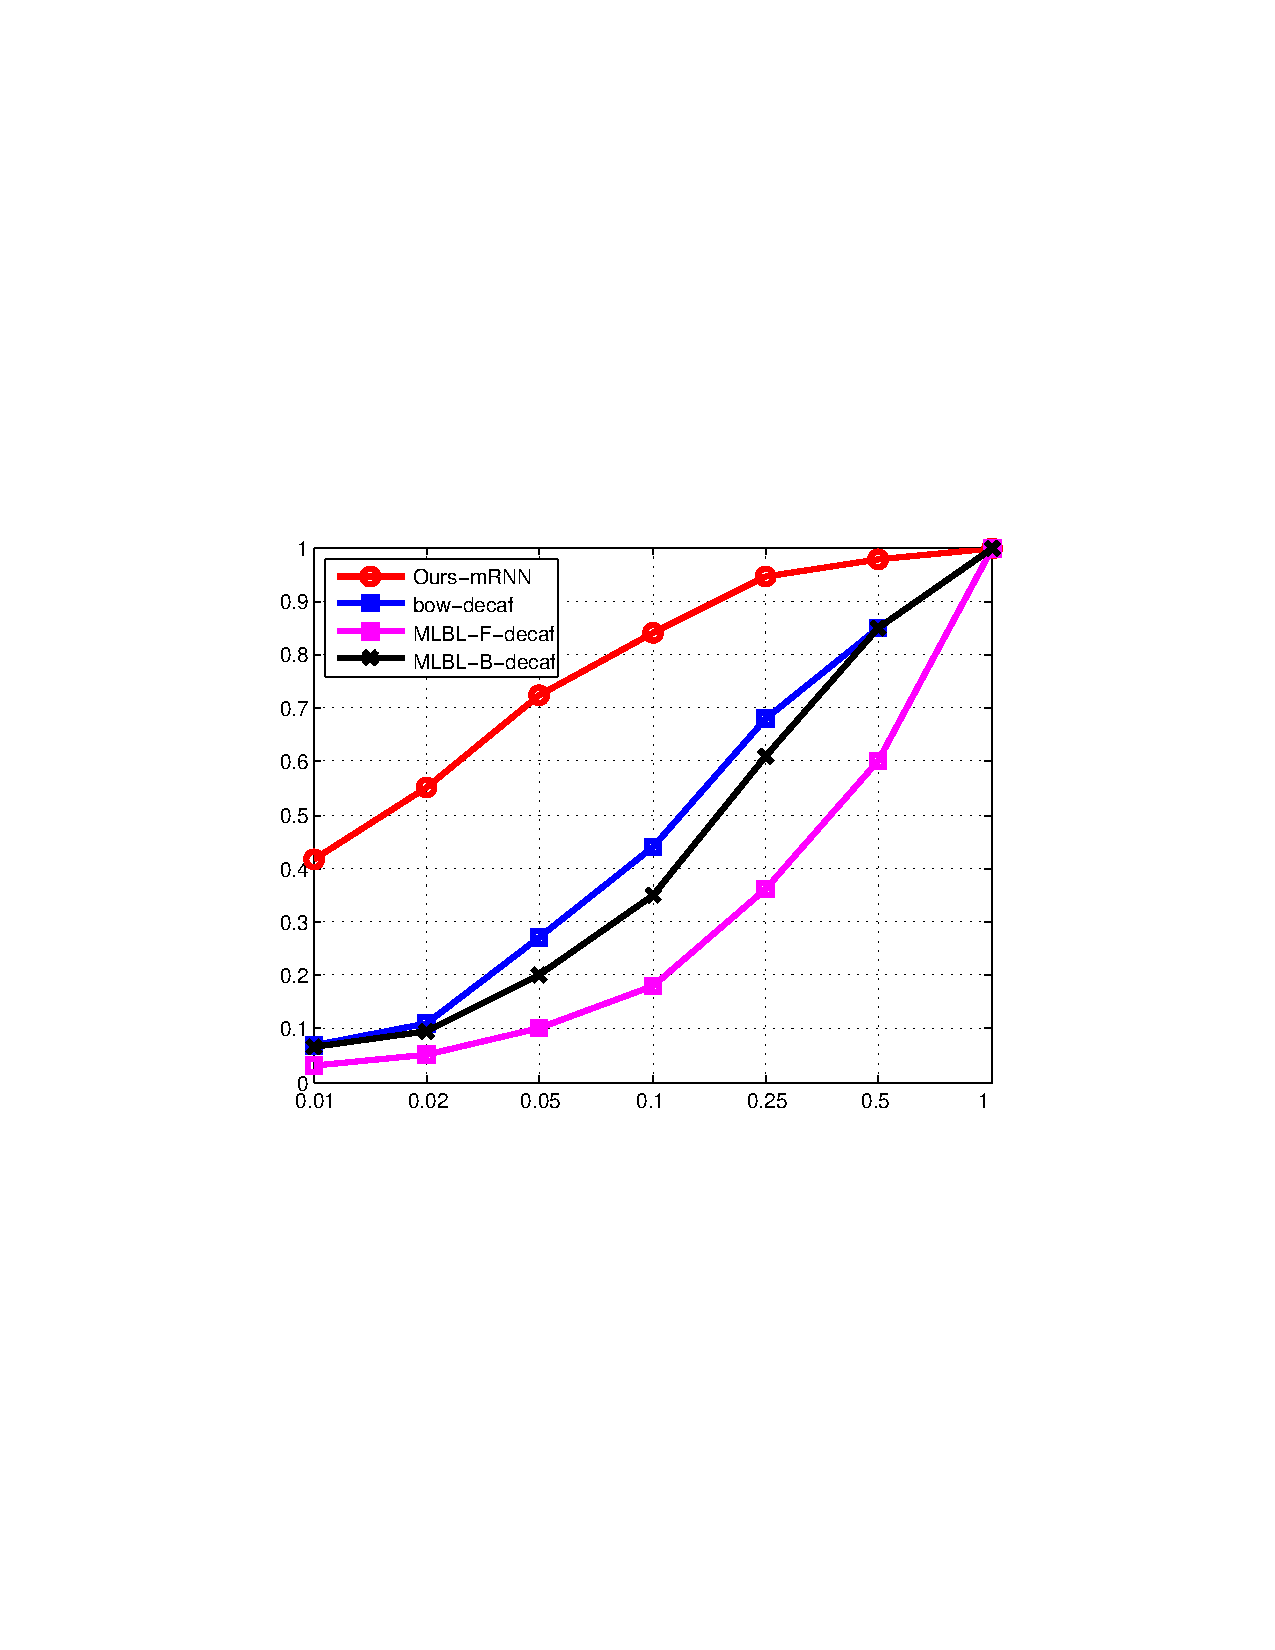
\includegraphics[width=\textwidth]{PaperFigures/I2T_iaprtc.pdf}
                \caption{Image to Text Curve}
        \end{subfigure}%
        ~ %add desired spacing between images, e. g. ~, \quad, \qquad, \hfill etc.
          %(or a blank line to force the subfigure onto a new line)
        \begin{subfigure}[b]{0.42\textwidth}
                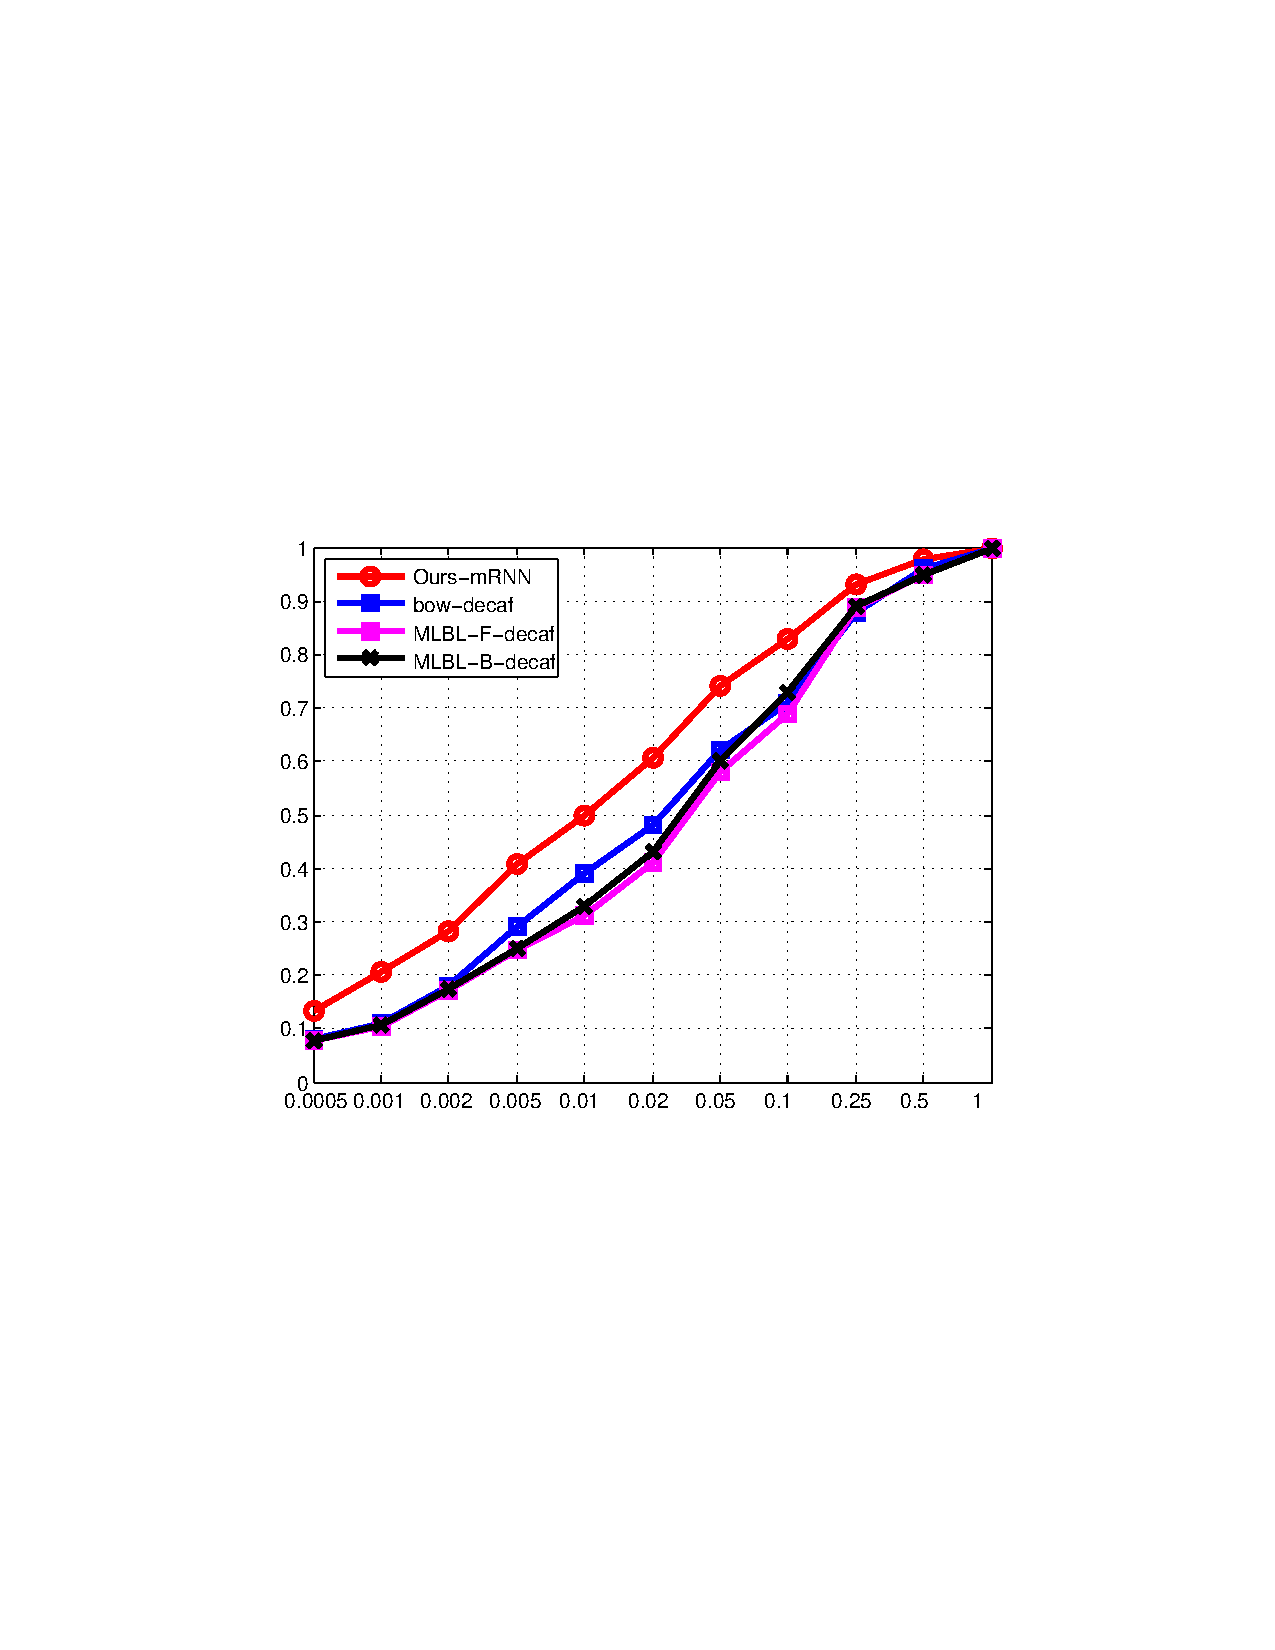
\includegraphics[width=\textwidth]{PaperFigures/T2I_iaprtc.pdf}
                \caption{Text to Image Curve}
        \end{subfigure}
        \caption{Retrieval recall curve for (a). Sentence retrieval task (b). Image retrieval task on IAPR TC-12 dataset. The behavior on the far left (i.e. top few retrievals) is most important.}
        \label{fig:iaprtc_ret_curve}
\end{figure}

\begin{table}[htb]
	\centering
\begin{tabular}{l|cccc|cccc}
\hline
      & \multicolumn{4}{c|}{Sentence Retrival (Image to Text)} & \multicolumn{4}{c}{Image Retrival (Text to Image)} \\
\hline
      & R@1   & R@5   & R@10  & Med r & R@1   & R@5   & R@10  & Med r \\
\hline
Ours-m-RNN & 20.9  & 43.8  & 54.4  & 8     & 13.2  & 31.2  & 40.8  & 21 \\
\hline
\end{tabular}%
	\caption{R@K and median rank (Med r) for iaprtc-12 dataset.}
	\label{tab:iaprtc_ret}
\end{table}

\subsection{Results on flickr8K}

This dataset was widely used as a benchmark dataset of image and sentence retrieval.
The R@K and Med r of different methods are shown in Table \ref{tab:flickr8K_ret}.
Our model outperforms the state-of-the-art methods (i.e Socher-decaf, DeViSE-decaf, DeepFE-decaf) by a large margin when using the same image features (i.e. decaf features).
% In a recent work \cite{karpathy2014fragment}, they showed that using more sophisticated image features (e.g. decaf feature combined with detection results), will increase the performance.
We also list the performance of methods using more sophisticated features in Table \ref{tab:flickr8K_ret}.
``-avg-rcnn'' denotes methods with features of the average CNN activation of all objects above a detection confidence threshold.
DeepFE-rcnn \cite{karpathy2014fragment} uses a fragment mapping strategy to better exploit the object detection results.
The results show that using these features will improve the performance.
Even without the help from the object detection methods, however, our method performs better than these methods in most of the evaluation metrics.
We will develop our framework using better image features in the future work.

\begin{table}[htb]
	\centering
\begin{tabular}{l|cccc|cccc}
\hline
      & \multicolumn{4}{c|}{Sentence Retrival (Image to Text)} & \multicolumn{4}{c}{Image Retrival (Text to Image)} \\
\hline
      & R@1   & R@5   & R@10  & Med r & R@1   & R@5   & R@10  & Med r \\
\hline
Random & 0.1   & 0.5   & 1.0   & 631   & 0.1   & 0.5   & 1.0   & 500 \\
Socher-decaf \cite{socher2014grounded} & 4.5   & 18.0  & 28.6  & 32    & 6.1   & 18.5  & 29.0  & 29 \\
Socher-avg-rcnn \cite{socher2014grounded} & 6.0   & 22.7  & 34.0  & 23    & 6.6   & 21.6  & 31.7  & 25 \\
DeViSE-avg-rcnn \cite{frome2013devise} & 4.8   & 16.5  & 27.3  & 28    & 5.9   & 20.1  & 29.6  & 29 \\
DeepFE-decaf \cite{karpathy2014fragment} & 5.9   & 19.2  & 27.3  & 34    & 5.2   & 17.6  & 26.5  & 32 \\
DeepFE-rcnn \cite{karpathy2014fragment} & 12.6  & 32.9  & 44.0  & 14    & 9.7   & 29.6  & \textbf{42.5} & \textbf{15} \\
Ours-m-RNN-decaf & \textbf{14.5} & \textbf{37.2} & \textbf{48.5} & \textbf{11} & \textbf{11.5} & \textbf{31.0} & 42.4  & \textbf{15}\\
\hline
\end{tabular}%
	\caption{Results of R@K and median rank (Med r) for Flickr8K dataset. Note DeepFE-rcnn uses more sophisticated image features than we do}
	\label{tab:flickr8K_ret}
\end{table}

We report the results of generated sentences in Table \ref{tab:flickr8_30K_gen}.
There is no publicly available algorithm that reported results on this dataset.
So we compared our m-RNN model with the Ours-RNN-Base model.
The m-RNN model performs much better than this baseline both in terms of the perplexity and BLEU scores.

%\begin{table}[htb]
%	\centering
%\begin{tabular}{l|cccc}
%\hline
%      & PERP  & B-1   & B-2   & B-3 \\
%\hline
%Ours-RNN-Base & 30.39 & 0.4383 & 0.1849 & 0.1339 \\
%Ours-m-RNN & \textbf{24.39} & \textbf{0.5778} & \textbf{0.2751} & \textbf{0.2307} \\
%\hline
%\end{tabular}%
%	\caption{Results of generated sentences in the flickr8K dataset. }
%	\label{tab:flickr8K_gen}
%\end{table}

\subsection{Results on flickr30K}

This dataset is a new dataset and there are only a few methods report their retrieval results on it so far.
We first show the R@K evaluation metric in Table \ref{tab:flickr30K_ret}.
Our method outperforms the state-of-the-art methods in most of the evaluation metrics.
The results of the sentence generation task with a comparison of our RNN baseline are shown in Table \ref{tab:flickr8_30K_gen}.

\vspace{-0.5em}
\begin{table}[htb]
	\centering
\begin{tabular}{l|cccc|cccc}
\hline
      & \multicolumn{4}{c|}{Sentence Retrival (Image to Text)} & \multicolumn{4}{c}{Image Retrival (Text to Image)} \\
\hline
      & R@1   & R@5   & R@10  & Med r & R@1   & R@5   & R@10  & Med r \\
Random & 0.1   & 0.6   & 1.1   & 631   & 0.1   & 0.5   & 1.0   & 500 \\
DeViSE-avg-rcnn \cite{frome2013devise} & 4.8   & 16.5  & 27.3  & 28    & 5.9   & 20.1  & 29.6  & 29 \\
DeepFE-rcnn \cite{karpathy2014fragment} & 16.4  & \textbf{40.2} & \textbf{54.7} & \textbf{8} & 10.3  & \textbf{31.4} & \textbf{44.5} & \textbf{13} \\
Ours-m-RNN-decaf & \textbf{18.4} & \textbf{40.2} & 50.9  & 10    & \textbf{12.6} & 31.2  & 41.5  & 16 \\
\hline
\end{tabular}%
\vspace{-0.3em}
	\caption{Results of R@K and median rank (Med r) for Flickr30K dataset.}
	\label{tab:flickr30K_ret}
\end{table}

%\begin{table}[h]
%	\centering
%\begin{tabular}{l|cccc}
%\hline
%      & PERP  & B-1   & B-2   & B-3 \\
%\hline
%Ours-RNN-Base & 43.96 & 0.4699 & 0.1964 & 0.1252 \\
%Ours-m-RNN & \textbf{35.11} & \textbf{0.5479} & \textbf{0.2392} & \textbf{0.1952} \\
%\hline
%\end{tabular}%
%	\caption{Results of generated sentences in the flickr8K dataset. }
%	\label{tab:flickr30K_gen}
%\end{table}

\begin{table}[htb]
	\centering
\begin{tabular}{l|rrrr|rrrr}
\hline
      & \multicolumn{4}{c|}{Flickr 8K} & \multicolumn{4}{c}{Flickr 30K} \\
\hline
      & $\mathcal{PPL}$  & B-1   & B-2   & B-3   & $\mathcal{PPL}$  & B-1   & B-2   & B-3 \\
\hline
Ours-RNN-Base & 30.39 & 0.4383 & 0.1849 & 0.1339 & 43.96 & 0.4699 & 0.1964 & 0.1252 \\
Ours-m-RNN & \textbf{24.39} & \textbf{0.5778} & \textbf{0.2751} & \textbf{0.2307} & \textbf{35.11} & \textbf{0.5479} & \textbf{0.2392} & \textbf{0.1952} \\
\hline
\end{tabular}%
\caption{Results of generated sentences in the Flickr8K and Flickr 30K dataset. }
\label{tab:flickr8_30K_gen}
\end{table}
